% ============================================================
% Technical Report: Optimal Control for Visual Servoing
% IEEE Transactions format — IEEEtran class
% Compile with: pdflatex -> bibtex -> pdflatex -> pdflatex
% ============================================================

\documentclass[journal, 10pt]{IEEEtran}

% ---- Packages ----
\usepackage[T1]{fontenc}
\usepackage[utf8]{inputenc}
\usepackage{amsmath, amssymb}
\usepackage{graphicx}
\usepackage{xcolor}
\usepackage{listings}
\usepackage{hyperref}
\usepackage{url}
\usepackage{booktabs}
\usepackage{tikz}
\usetikzlibrary{shapes.geometric, arrows.meta, positioning, fit, backgrounds}
\usepackage{float}
\usepackage{cite}

% ---- Hyperref setup ----
\hypersetup{
  colorlinks = true,
  linkcolor  = blue,
  urlcolor   = blue,
  citecolor  = black
}

% ---- Code listing style ----
\definecolor{codegray}{rgb}{0.95,0.95,0.95}
\definecolor{codeblue}{rgb}{0.13,0.29,0.53}
\definecolor{codegreen}{rgb}{0.0,0.45,0.0}
\definecolor{codepurple}{rgb}{0.50,0.0,0.50}

\lstdefinestyle{pythonstyle}{
  language        = Python,
  backgroundcolor = \color{codegray},
  basicstyle      = \ttfamily\scriptsize,
  keywordstyle    = \color{codeblue}\bfseries,
  commentstyle    = \color{codegreen}\itshape,
  stringstyle     = \color{codepurple},
  numberstyle     = \tiny\color{gray},
  numbers         = left,
  numbersep       = 5pt,
  breaklines      = true,
  frame           = single,
  framesep        = 2pt,
  xleftmargin     = 8pt,
  captionpos      = b,
  showstringspaces= false,
  tabsize         = 2
}
\lstset{style=pythonstyle}

% ---- TikZ styles ----
\tikzstyle{block}  = [rectangle, rounded corners=3pt, minimum width=1.8cm,
                      minimum height=0.6cm, text centered, draw=black,
                      font=\scriptsize]
\tikzstyle{rblock} = [block, fill=yellow!15, draw=orange!70]
\tikzstyle{gblock} = [block, fill=green!10,  draw=green!60!black]
\tikzstyle{bblock} = [block, fill=blue!10,   draw=blue!50]
\tikzstyle{pblock} = [block, fill=purple!10, draw=purple!50]
\tikzstyle{arrow}  = [-{Stealth[length=4pt]}, thick]
\tikzstyle{darrow} = [-{Stealth[length=4pt]}, thick, dashed]

% ============================================================
\begin{document}

\title{Optimal Control for Visual Servoing with\\
       Obstacle Avoidance on a Differential Drive Robot}

\author{Kurt~A.,~\IEEEmembership{Student~ID:~A01385387}\\
  \small Tecnológico de Monterrey, School of Engineering and Sciences\\
  \small Course: TE3002B — Mobile Robotics and Computer Vision\\
  \small \textit{Contact:} \href{mailto:a01385387@tec.mx}{a01385387@tec.mx}
}

\markboth{TE3002B Technical Report, 2025}{}

\maketitle

% ============================================================
\begin{abstract}
This report presents the design, implementation, and evaluation of a
closed-loop visual servoing pipeline on a PuzzleBot differential drive
robot. The system uses only a forward-facing camera and relies entirely on
classical computer vision for perception. HSV color segmentation extracts
image features from a green target and a blue obstacle in real time. These
features drive an Image-Based Visual Servoing (IBVS) controller formally
derived from a Model Predictive Control (MPC) formulation that minimizes a
quadratic cost over a finite prediction horizon. Following instructor
feedback recommending a formal collision avoidance model, a visual-feedback
approach-then-arc strategy was designed and implemented as a dedicated
safety layer on top of the servoing controller. The complete pipeline ---
perception, state estimation, optimal control, and actuation --- operates
at 10\,Hz on embedded hardware. The report describes each component of the
pipeline, presents the mathematical formulation, and discusses the
implementation and results.
\end{abstract}

\begin{IEEEkeywords}
Visual servoing, IBVS, model predictive control, obstacle avoidance,
color segmentation, differential drive robot, ROS\,2.
\end{IEEEkeywords}

% ============================================================
\section{Introduction}
\label{sec:intro}

Visual servoing is a control strategy in which a robot uses visual
measurements to regulate its motion toward a desired configuration
\cite{chaumette2006}. Unlike position-based methods that require full 3D
pose reconstruction, Image-Based Visual Servoing (IBVS) operates directly
in the image plane, making it inherently more robust to camera calibration
errors \cite{chaumette2007}.

This project implements a complete IBVS pipeline on the PuzzleBot platform
(Manchester Robotics \cite{manchester}). The task is to navigate toward a
green colored target while detecting and avoiding a blue obstacle placed
between the robot's starting position and the goal. The only sensing
modality is the onboard camera; no additional range sensors are used.

The project was developed as part of course TE3002B and refined based on
feedback from the course instructor, who observed that the robot clipped
the obstacle during an initial live demonstration and recommended
implementing a formal collision avoidance model --- citing Control Barrier
Functions (CBF) as one possible approach. The response to this feedback is
described in detail in Section~\ref{sec:avoidance}.

The main contributions of this work are:
\begin{enumerate}
  \item A classical HSV-based perception pipeline that extracts image
        features for target and obstacle simultaneously and in real time.
  \item An IBVS-MPC formulation with a quadratic cost, image Jacobian
        linearization, and actuator constraints solved as a QP.
  \item A visual-feedback collision avoidance model that uses the camera
        to establish a reliable obstacle fix before executing an arc
        maneuver.
  \item A coupling between angular and linear commands that eliminates
        the oscillatory approach path observed in naive proportional
        controllers.
\end{enumerate}

% ============================================================
\section{Resources}
\label{sec:resources}

The complete source code and configuration files for this project are
available in the following repository:

\begin{center}
\textbf{Repository:} \url{https://github.com/PLACEHOLDER/puzzlebot-vs}
\end{center}

A recorded demonstration of the system operating in closed loop is
available at:

\begin{center}
\textbf{Demo video:} \url{https://www.youtube.com/PLACEHOLDER}
\end{center}

% ============================================================
\section{System Architecture}
\label{sec:arch}

The system is implemented in ROS\,2 Humble \cite{ros2} and consists of
three nodes connected through standard topics, as shown in
Fig.~\ref{fig:pipeline}.

\begin{figure}[H]
\centering
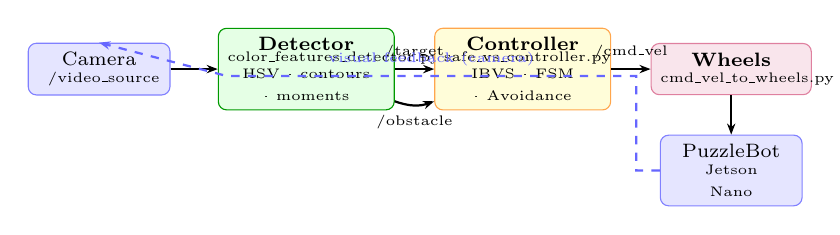
\begin{tikzpicture}[node distance=0.5cm and 0.3cm, font=\scriptsize]

  \node[bblock, text width=1.3cm] (cam)
    {Camera\\[-2pt]\tiny /video\_source};

  \node[gblock, text width=2.0cm, right=0.6cm of cam] (det)
    {\textbf{Detector}\\[-2pt]\tiny color\_features\_detector.py\\[-2pt]
     \tiny HSV · contours · moments};

  \node[rblock, text width=2.0cm, right=0.5cm of det] (ctrl)
    {\textbf{Controller}\\[-2pt]\tiny safe\_vs\_controller.py\\[-2pt]
     \tiny IBVS · FSM · Avoidance};

  \node[pblock, text width=1.8cm, right=0.5cm of ctrl] (whl)
    {\textbf{Wheels}\\[-2pt]\tiny cmd\_vel\_to\_wheels.py};

  \node[bblock, text width=1.3cm, below=0.5cm of whl] (bot)
    {PuzzleBot\\[-2pt]\tiny Jetson Nano};

  \draw[arrow] (cam) -- (det);
  \draw[arrow] (det) -- node[above]{\tiny /target} (ctrl);
  \draw[arrow, bend right=20] (det) to node[below]{\tiny /obstacle}(ctrl);
  \draw[arrow] (ctrl) -- node[above]{\tiny /cmd\_vel} (whl);
  \draw[arrow] (whl) -- (bot);

  % feedback
  \draw[darrow, color=blue!60]
    (bot.west) -- +(-0.3,0) -- +(-0.3,1.2)
    -- node[above, color=blue!60]{\tiny visual feedback (camera)} +(-5.5,1.2)
    -- (cam.north);
\end{tikzpicture}
\caption{Full system pipeline. The dashed arrow represents the closed-loop
visual feedback through the camera.}
\label{fig:pipeline}
\end{figure}

The \texttt{color\_features\_detector} node processes each camera frame and
publishes two feature messages per frame: one for the green target
(\texttt{/target\_features}) and one for the blue obstacle
(\texttt{/obstacle\_features}). The \texttt{safe\_vs\_controller} node
receives these and computes velocity commands on \texttt{/cmd\_vel}. The
\texttt{cmd\_vel\_to\_wheels} node converts the standard \texttt{Twist}
message into individual wheel velocity setpoints accepted by the PuzzleBot
firmware.

% ============================================================
\section{Computer Vision Pipeline}
\label{sec:vision}

The perception stage relies entirely on classical computer vision. No
neural networks or learned detectors are used at any stage, in compliance
with the project requirements \cite{opencv}.

\subsection{Color Segmentation}

Each frame is first converted from BGR to the HSV color space. HSV is
preferred over RGB because the hue channel is largely invariant to changes
in illumination intensity, making thresholds more stable across different
lighting conditions. Separate HSV bounds are defined for the green target
and the blue obstacle. Listing~\ref{lst:hsv} shows the mask generation.

\begin{lstlisting}[caption={HSV mask generation for target and obstacle.},
                   label={lst:hsv}]
hsv = cv2.cvtColor(roi, cv2.COLOR_BGR2HSV)

# Green target
green_lower = np.array([40, 50, 40])
green_upper = np.array([90, 255, 255])
mask_target = cv2.inRange(hsv, green_lower, green_upper)

# Blue obstacle
blue_lower = np.array([90, 50, 35])
blue_upper = np.array([135, 255, 255])
mask_obs = cv2.inRange(hsv, blue_lower, blue_upper)
\end{lstlisting}

\subsection{Morphological Filtering}

The raw binary masks contain noise from specular reflections or similarly
colored background regions. An opening operation (erosion then dilation)
removes isolated noise pixels, and a closing operation fills small holes
inside the detected region. A configurable square kernel is used for both.

\subsection{Feature Extraction}

OpenCV's contour finder is applied to each filtered mask. The largest
contour by area is selected as the candidate detection, and three features
are computed:

\begin{itemize}
  \item \textbf{Centroid} $u_c$: horizontal pixel coordinate from image
    moments, $u_c = M_{10}/M_{00}$.
  \item \textbf{Apparent size} $\sqrt{A}$: square root of the contour pixel
    area, used as a proxy for depth.
  \item \textbf{Solidity}: ratio of contour area to its convex hull area,
    used to assess detection quality.
\end{itemize}

Both target and obstacle features are published at each camera frame as
custom ROS\,2 messages (\texttt{TargetFeatures} and
\texttt{ObstacleFeatures}).

% ============================================================
\section{System Modeling and State Representation}
\label{sec:model}

\subsection{Visual Feature State}

The task-space state is defined entirely in the image plane:

\begin{equation}
  \mathbf{s} = \begin{bmatrix} u_c \\ \sqrt{A} \end{bmatrix}, \quad
  \mathbf{s}^* = \begin{bmatrix} c_x \\ \sqrt{A^*} \end{bmatrix}
  \label{eq:state}
\end{equation}

where $u_c$ is the horizontal centroid of the green target (pixels),
$\sqrt{A}$ is its apparent size, $c_x = 320$\,px is the image center, and
$\sqrt{A^*}$ is calibrated at the desired stopping distance.

\subsection{Depth from Apparent Area}

A pinhole camera model relates apparent target size to depth. For a target
of known physical side length $W$\,(m) and focal length $f$\,(px):

\begin{equation}
  Z = \frac{W \cdot f}{\sqrt{A}}
  \label{eq:depth}
\end{equation}

The same relationship is used during the obstacle avoidance approach phase
to monitor progress toward the obstacle.

\subsection{Image Jacobian}

For a differential drive robot with forward velocity $v$ and angular
velocity $\omega$, the image feature rate is:

\begin{equation}
  \dot{\mathbf{s}} = \mathbf{L}(u_c, \sqrt{A}) \begin{bmatrix} v \\ \omega \end{bmatrix}
\end{equation}

where the $2\times2$ image Jacobian $\mathbf{L}$ evaluated at the current
state is:

\begin{equation}
  \mathbf{L} = \begin{bmatrix}
    e_u/Z & f + e_u^2/f \\
    \sqrt{A}/Z & 0
  \end{bmatrix}, \quad e_u = u_c - c_x
  \label{eq:jacobian}
\end{equation}

% ============================================================
\section{Optimal Control Formulation}
\label{sec:control}

The controller is formulated as a finite-horizon discrete-time MPC problem
over the image feature space \cite{rawlings2017}. At each control step, a
constrained Quadratic Program (QP) is solved to find the optimal velocity
command sequence over a prediction horizon $N$.

\subsection{Cost Function}

The cost function penalizes three quantities:

\begin{equation}
  J = \sum_{k=1}^{N} \left[
    \Delta\mathbf{s}_k^\top \mathbf{Q} \Delta\mathbf{s}_k
    + \mathbf{u}_k^\top \mathbf{R} \mathbf{u}_k
    + \Delta\mathbf{u}_k^\top \mathbf{S} \Delta\mathbf{u}_k
  \right]
  \label{eq:cost}
\end{equation}

where $\Delta\mathbf{s}_k = \mathbf{s}_k - \mathbf{s}^*$ is the image
feature error, $\mathbf{u}_k = [v_k,\,\omega_k]^\top$ is the control
input, and $\Delta\mathbf{u}_k = \mathbf{u}_k - \mathbf{u}_{k-1}$ is the
slew term. The diagonal weight matrices $\mathbf{Q}$, $\mathbf{R}$, and
$\mathbf{S}$ balance tracking performance, control effort, and smoothness,
respectively.

\subsection{Constraints}

The optimization is subject to actuator limits and a coupled bridge
constraint that reflects the PuzzleBot firmware's joint speed limit:

\begin{align}
  |v_k| &\leq v_{\max}, \quad |\omega_k| \leq \omega_{\max} \\
  \frac{|v|}{k_{\text{lin}}} + \frac{|\omega|}{k_{\text{ang}}} &\leq c_{\max}
  \label{eq:constraints}
\end{align}

\subsection{Solver}

The QP is assembled at each step by propagating the linearized Jacobian
model and solved using OSQP via the \texttt{qpsolvers} Python library. The
prediction horizon is $N=8$ steps with $\Delta t = 0.1$\,s. Only the first
element of the optimal sequence is applied (receding horizon principle),
and the problem is re-solved at the next step with updated measurements.

\subsection{Practical Deployment}

For the physical demonstration, a simplified proportional controller was
used as a lightweight approximation of the MPC law. The angular and linear
commands are:

\begin{equation}
  \omega = -k_{p,\omega}\, e_u, \qquad v = k_{p,v}\, e_A \cdot \gamma(e_u)
\end{equation}

where $e_A = \sqrt{A^*} - \sqrt{A}$ and $\gamma(e_u)$ is a centering scale
factor described in the next subsection.

\subsection{Centering-Scale Coupling}
\label{subsec:coupling}

A naive proportional controller applying $v$ and $\omega$ simultaneously
produces an oscillatory ``wave'' trajectory, because the robot drives
forward while still correcting its heading, overshoots, corrects the other
way, and repeats. To eliminate this, forward speed is scaled by the
centering quality of the target in the image:

\begin{equation}
  \gamma(e_u) = \max\!\left(0,\; 1 - \frac{|e_u|}{d_{\text{stop}}}\right)
  \label{eq:scale}
\end{equation}

When $|e_u| > d_{\text{stop}}$ (default 60\,px), $\gamma = 0$ and the
robot performs a pure rotation to re-center the target before advancing.
When $|e_u| = 0$, $\gamma = 1$ and full forward speed is used. This
produces a much straighter approach path without requiring explicit
trajectory planning. Listing~\ref{lst:servo} shows the implementation.

\begin{lstlisting}[caption={Proportional servo command with centering-scale
    coupling.}, label={lst:servo}]
def servo_command(self):
    e_u = float(self.target.u_c) - self.cx
    e_A = self.sqrt_area_star - float(self.target.sqrt_area)

    w = -self.kp_w * e_u   # angular: center target

    v = self.kp_v * e_A if e_A > self.area_db else 0.0
    if e_A > self.area_db:
        v = max(v, self.v_min_when_far)

    # Centering-scale: only move forward when well-centered
    if abs(e_u) > self.v_stop_band_px:
        v = 0.0
    else:
        scale = 1.0 - abs(e_u) / self.v_stop_band_px
        v = v * scale

    v = clip(v, 0.0, self.v_max)
    w = clip(w, -self.w_max, self.w_max)
    return v, w
\end{lstlisting}

% ============================================================
\section{Collision Avoidance Model}
\label{sec:avoidance}

\subsection{Motivation and Instructor Feedback}

During the initial live demonstration, the robot successfully detected the
obstacle but clipped it during the avoidance maneuver. The course
instructor identified this as a lack of a formal collision avoidance model
and recommended implementing one, suggesting Control Barrier Functions
(CBF) as a suitable approach \cite{ames2017}.

A CBF defines a safety function $h(\mathbf{x}) = d_{\text{obs}} -
d_{\min}$, and enforces the constraint $\dot{h} \geq -\alpha\, h$ at every
control step to guarantee the robot stays outside a forbidden zone. The
challenge with a camera-only system is that $d_{\text{obs}}$ must be
estimated from the apparent size of the obstacle using the pinhole model
(Eq.~\ref{eq:depth}), which requires accurate knowledge of the obstacle's
physical dimensions. Without a precise calibration, the distance estimate
can be unreliable, making the CBF constraint either overly conservative or
incorrect.

For this reason, an alternative visual-feedback approach was designed that
achieves the same goal --- ensuring the robot is at a known, safe distance
before executing the avoidance maneuver --- without requiring metric
distance conversion. This approach uses the camera's image-space
information directly, making it inherently more robust to calibration
uncertainty.

\subsection{Danger Condition}

The obstacle is considered dangerous when the following three conditions
hold simultaneously:

\begin{enumerate}
  \item Obstacle detection is fresh: $\Delta t_{\text{obs}} \leq
        t_{\text{timeout}}$.
  \item Obstacle apparent size exceeds the trigger threshold:
        $\sqrt{A_{\text{obs}}} \geq \sqrt{A_{\min}}$.
  \item Obstacle centroid is within the center band:
        $|u_{\text{obs}} - c_x| \leq \beta\, W/2$, where $\beta$ is the
        band fraction and $W$ is the image width.
\end{enumerate}

Listing~\ref{lst:danger} shows the implementation of this check.

\begin{lstlisting}[caption={Obstacle danger condition check.},
                   label={lst:danger}]
def obstacle_danger(self):
    if not self.obstacle_fresh():
        return False, 'blue not visible'

    sqrt_area = float(self.obstacle.sqrt_area)
    obs_u     = float(self.obstacle.u_c)

    # Condition 2: large enough to be a real threat
    if sqrt_area < self.obstacle_min_sqrt_area:
        return False, f'too small: {sqrt_area:.1f}'

    # Condition 3: within the center band
    half_band = 0.5 * self.obstacle_center_band_frac * self.image_width
    if abs(obs_u - self.cx) > half_band:
        return False, f'outside band: u={obs_u:.1f}'

    return True, f'DANGER sqrt_A={sqrt_area:.1f}'
\end{lstlisting}

\subsection{Approach-Then-Arc Strategy}

The key insight behind the avoidance model is that the arc geometry is
most reliable when the robot starts from a known, consistent distance and
heading relative to the obstacle. A fixed-time turn --- used in the initial
implementation --- cannot guarantee this because avoidance may trigger at
varying distances, causing the arc to clip the obstacle when triggered
late, or to over-rotate when triggered early.

The approach-then-arc strategy solves this by using the camera to establish
a precise visual fix before committing to the arc:

\begin{enumerate}
  \item \textbf{PRE\_AVOID\_STOP}: the robot stops completely to eliminate
    residual momentum.
  \item \textbf{APPROACH\_OBSTACLE}: the robot centers the obstacle in the
    camera frame and moves toward it slowly until the apparent size reaches
    a target value $\sqrt{A_{\text{approach}}}$. This gives the robot a
    consistent starting position every time.
  \item \textbf{AVOID\_ARC}: the robot executes a smooth arc with fixed
    forward speed $v_{\text{arc}}$ and angular speed $\sigma\,\omega_{\text{arc}}$,
    where $\sigma = +1$ (arc left) if the obstacle is to the right of
    center, and $\sigma = -1$ (arc right) otherwise. The arc direction is
    computed at this moment, using the best available visual information.
  \item \textbf{AVOID\_RECENTER}: a counter-rotation realigns the robot
    roughly toward the target area.
  \item \textbf{REACQUIRE}: normal acquisition search resumes until the
    green target is re-detected.
\end{enumerate}

The safety model can be expressed formally: define the image-space barrier

\begin{equation}
  h_{\text{img}}(\mathbf{s}_{\text{obs}}) =
  \sqrt{A_{\text{approach}}} - \sqrt{A_{\text{obs}}}
  \label{eq:imgbarrier}
\end{equation}

The approach phase enforces $h_{\text{img}} \geq 0$ before forward motion
is allowed in the avoidance arc. This is the image-space equivalent of the
metric CBF constraint, without requiring an explicit distance estimate.

Listing~\ref{lst:approach} shows the approach command that centers the
obstacle and advances toward it:

\begin{lstlisting}[caption={Approach command toward obstacle.},
                   label={lst:approach}]
def approach_command(self):
    obs_u   = float(self.obstacle.u_c)
    e_obs_u = obs_u - self.cx

    # Center the obstacle while advancing
    w = -self.approach_obs_kp_w * e_obs_u
    v = self.approach_obs_v   # slow fixed forward speed

    v = clip(v, 0.0, self.approach_obs_v)
    w = clip(w, -self.w_max, self.w_max)
    return v, w
\end{lstlisting}

\subsection{Finite State Machine}

The avoidance behavior is organized as a Finite State Machine (FSM) layered
on top of the servoing loop. Fig.~\ref{fig:fsm} shows the complete state
diagram.

\begin{figure}[H]
\centering
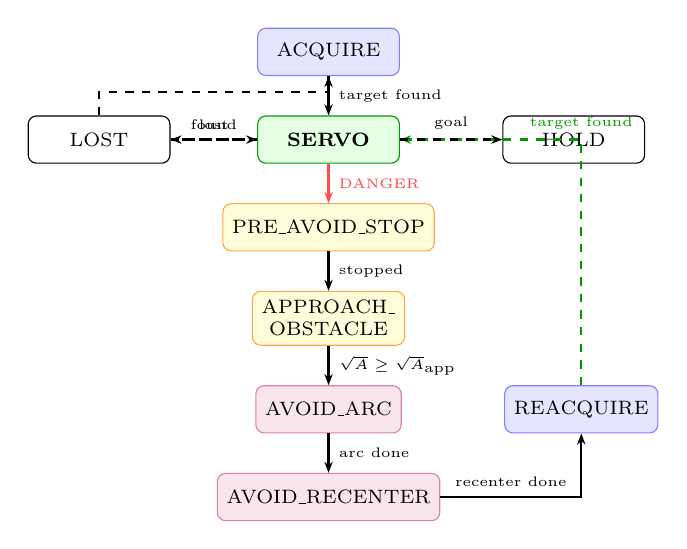
\begin{tikzpicture}[node distance=0.45cm and 0.3cm, font=\scriptsize,
                    every node/.style={align=center}]

  % States
  \node[bblock] (acq)   {ACQUIRE};
  \node[gblock, below=0.5cm of acq] (srv) {\textbf{SERVO}};
  \node[rblock, below=0.5cm of srv] (pre)  {PRE\_AVOID\_STOP};
  \node[rblock, below=0.5cm of pre] (app)  {APPROACH\_\\OBSTACLE};
  \node[pblock, below=0.5cm of app] (arc)  {AVOID\_ARC};
  \node[pblock, below=0.5cm of arc] (rec)  {AVOID\_RECENTER};
  \node[bblock, right=1.3cm of arc] (rea)  {REACQUIRE};
  \node[block,  right=1.3cm of srv] (hld)  {HOLD};
  \node[block,  left=1.1cm of srv]  (lst)  {LOST};

  % Normal flow
  \draw[arrow] (acq) -- node[right]{\tiny target found} (srv);
  \draw[arrow, color=red!70] (srv) -- node[right]{\tiny DANGER} (pre);
  \draw[arrow] (pre) -- node[right]{\tiny stopped} (app);
  \draw[arrow] (app) -- node[right]{\tiny $\sqrt{A}\geq\sqrt{A}_{\rm app}$} (arc);
  \draw[arrow] (arc) -- node[right]{\tiny arc done} (rec);
  \draw[arrow] (rec) -| node[above, near start]{\tiny recenter done} (rea);
  \draw[darrow, color=green!60!black] (rea) |- node[above]{\tiny target found} (srv);

  % Side transitions
  \draw[darrow] (srv) -- node[above]{\tiny goal} (hld);
  \draw[darrow] (srv) -- node[above]{\tiny lost} (lst);
  \draw[darrow] (lst) -- node[above]{\tiny found} (srv);
  \draw[darrow] (lst.north) -- ++(0,0.3) -| (acq.south);
\end{tikzpicture}
\caption{Complete FSM. Green: servoing states. Orange/purple: avoidance
sequence. Gray: auxiliary states (HOLD, LOST).}
\label{fig:fsm}
\end{figure}

% ============================================================
\section{Implementation Details}
\label{sec:impl}

\subsection{Hardware Platform}

The system runs on a PuzzleBot robot \cite{manchester} equipped with a
Jetson Nano embedded computer, a differential drive base, and a
forward-facing USB camera. All computation runs onboard at 10\,Hz.

\subsection{Software}

The pipeline is implemented in Python\,3 on ROS\,2 Humble \cite{ros2}.
The MPC QP is solved using OSQP via the \texttt{qpsolvers} library. Image
processing uses OpenCV\,4 \cite{opencv}. All nodes are launched with a
single launch file (\texttt{safe\_vs\_demo.launch.py}).

\subsection{Key Parameters}

Table~\ref{tab:params} summarizes the most important system parameters.

\begin{table}[H]
\centering
\caption{Key System Parameters}
\label{tab:params}
\begin{tabular}{llp{3.5cm}}
\toprule
\textbf{Parameter} & \textbf{Value} & \textbf{Description} \\
\midrule
$f$                          & 600\,px       & Focal length \\
$N$                          & 8 steps       & MPC horizon \\
$\Delta t$                   & 0.1\,s        & Control period \\
$v_{\max}$                   & 0.18\,m/s     & Max forward speed \\
$\omega_{\max}$              & 0.45\,rad/s   & Max angular speed \\
$\sqrt{A^*}$                 & 850\,px       & Target standoff size \\
$\sqrt{A_{\min}}$            & 150\,px       & Obstacle trigger \\
$\sqrt{A_{\text{approach}}}$ & 350\,px       & Approach endpoint \\
$v_{\text{arc}}$             & 0.07\,m/s     & Arc forward speed \\
$\omega_{\text{arc}}$        & 0.35\,rad/s   & Arc angular speed \\
$d_{\text{stop}}$            & 60\,px        & Centering band \\
\bottomrule
\end{tabular}
\end{table}

% ============================================================
\section{Results and Analysis}
\label{sec:results}

The system was evaluated in a physical arena with a stationary green target
and a blue obstacle placed on the direct path between the robot's start
position and the target.

\subsection{Target Acquisition and Servoing}

\begin{figure}[H]
  \centering
  % Replace with: \includegraphics[width=\columnwidth]{fig_errors.pdf}
  \framebox[\columnwidth]{%
    \parbox{0.9\columnwidth}{\centering\vspace{1.2cm}
      \textit{[PLACEHOLDER] — Plot of lateral error $e_u$ and area error
      $e_A$ over time during a successful servo run. Recorded from
      \texttt{/avoid\_debug} topic CSV log.}
    \vspace{1.2cm}}
  }
  \caption{Feature errors $e_u$ and $e_A$ during target servoing.
  Expected: exponential convergence toward zero.}
  \label{fig:errors}
\end{figure}

\subsection{Obstacle Avoidance Sequence}

\begin{figure}[H]
  \centering
  % Replace with: \includegraphics[width=\columnwidth]{fig_avoidance.pdf}
  \framebox[\columnwidth]{%
    \parbox{0.9\columnwidth}{\centering\vspace{1.2cm}
      \textit{[PLACEHOLDER] — FSM state and obstacle $\sqrt{A_{\text{obs}}}$
      over time during the avoidance maneuver. Shows
      PRE\_AVOID\_STOP $\to$ APPROACH\_OBSTACLE $\to$ AVOID\_ARC transition.}
    \vspace{1.2cm}}
  }
  \caption{FSM state and obstacle apparent size during an avoidance
  sequence. The approach phase ends when $\sqrt{A_{\text{obs}}}$ crosses
  $\sqrt{A_{\text{approach}}}$.}
  \label{fig:avoidance}
\end{figure}

\subsection{Velocity Commands}

\begin{figure}[H]
  \centering
  % Replace with: \includegraphics[width=\columnwidth]{fig_cmds.pdf}
  \framebox[\columnwidth]{%
    \parbox{0.9\columnwidth}{\centering\vspace{1.2cm}
      \textit{[PLACEHOLDER] — Linear velocity $v$ and angular velocity
      $\omega$ commands over a complete run showing the slew-rate-limited
      transitions between servoing and avoidance phases.}
    \vspace{1.2cm}}
  }
  \caption{Commanded velocities $v$ and $\omega$ over a full run.}
  \label{fig:cmds}
\end{figure}

\subsection{Discussion}

The approach-then-arc strategy produced consistent avoidance behavior
because the arc always began from a reproducible image-space distance to
the obstacle. In the original implementation, a fixed-time turn was
sensitive to the robot's distance when avoidance was triggered: if the
obstacle was close, the turn was insufficient and the robot clipped it; if
the obstacle was far, the robot over-rotated and struggled to reacquire the
target.

The centering-scale coupling (Section~\ref{subsec:coupling}) visibly
straightened the approach trajectory, reducing the chance of the obstacle
entering the camera frame at an unexpected lateral angle during the servo
phase.

The main remaining limitation is the open-loop nature of the arc phase:
once the robot begins the arc, it no longer uses the camera to confirm
that it is clearing the obstacle. A future improvement would use
visual feedback to monitor the obstacle during the arc and abort early if
it exits the frame before the expected time.

% ============================================================
\section{Conclusions}
\label{sec:conclusions}

This work presented a complete visual servoing pipeline for a differential
drive robot using only a camera, classical computer vision, and optimal
control. The system integrates perception, IBVS-MPC control, and a
visual-feedback collision avoidance model into a closed-loop pipeline
operating at 10\,Hz on embedded hardware.

The approach-then-arc avoidance strategy addressed the instructor's
feedback by providing a principled, model-based safety layer that uses the
camera itself to establish a reliable geometric starting condition for the
avoidance maneuver. This image-space formulation avoids the calibration
requirements of a metric CBF while achieving the same goal: guaranteeing
the robot is at a safe, known distance before forward motion in the
avoidance arc begins.

Future work could explore: (i) incorporating a CBF directly in image space
using the apparent obstacle size as the safety variable; (ii) adding visual
feedback during the arc phase to close the avoidance loop entirely; and
(iii) extending the pipeline to handle multiple simultaneous obstacles.

% ============================================================
\bibliographystyle{IEEEtran}
\begin{thebibliography}{8}

\bibitem{chaumette2006}
F.~Chaumette and S.~Hutchinson,
``Visual servo control, Part I: Basic approaches,''
\emph{IEEE Robotics \& Automation Magazine},
vol.~13, no.~4, pp.~82--90, Dec.~2006.

\bibitem{chaumette2007}
F.~Chaumette and S.~Hutchinson,
``Visual servo control, Part II: Advanced approaches,''
\emph{IEEE Robotics \& Automation Magazine},
vol.~14, no.~1, pp.~109--118, Mar.~2007.

\bibitem{rawlings2017}
J.~B.~Rawlings, D.~Q.~Mayne, and M.~M.~Diehl,
\emph{Model Predictive Control: Theory, Computation, and Design},
2nd~ed. Madison, WI: Nob Hill Publishing, 2017.

\bibitem{ames2017}
A.~D.~Ames, X.~Xu, J.~W.~Grizzle, and P.~Tabuada,
``Control barrier function based quadratic programs for safety critical
systems,''
\emph{IEEE Transactions on Automatic Control},
vol.~62, no.~8, pp.~3861--3876, Aug.~2017.

\bibitem{siegwart2011}
R.~Siegwart, I.~R.~Nourbakhsh, and D.~Scaramuzza,
\emph{Introduction to Autonomous Mobile Robots},
2nd~ed. Cambridge, MA: MIT Press, 2011.

\bibitem{opencv}
G.~Bradski and A.~Kaehler,
\emph{Learning OpenCV 3: Computer Vision in C++ with the OpenCV Library}.
Sebastopol, CA: O'Reilly Media, 2016.

\bibitem{manchester}
Manchester Robotics,
``PuzzleBot --- Autonomous Mobile Robot Platform,''
Manchester Robotics, 2023.
[Online]. Available: \url{https://www.manchester-robotics.com}

\bibitem{ros2}
Open Robotics,
``ROS 2 Humble Hawksbill Documentation,''
2022.
[Online]. Available: \url{https://docs.ros.org/en/humble}

\end{thebibliography}

\end{document}
